
\documentclass[a4paper,12pt]{article}
%%%%%%%%%%%%%%%%%%%%%%%%%%%%%%%%%%%%%%%%%%%%%%%%%%%%%%%%%%%%%%%%%%%%%%%%%%%%%%%%%%%%%%%%%%%%%%%%%%%%%%%%%%%%%%%%%%%%%%%%%%%%%%%%%%%%%%%%%%%%%%%%%%%%%%%%%%%%%%%%%%%%%%%%%%%%%%%%%%%%%%%%%%%%%%%%%%%%%%%%%%%%%%%%%%%%%%%%%%%%%%%%%%%%%%%%%%%%%%%%%%%%%%%%%%%%
\usepackage{eurosym}
\usepackage{vmargin}
\usepackage{amsmath}
\usepackage{graphics}
\usepackage{epsfig}
\usepackage{subfigure}
\usepackage{fancyhdr}

\setcounter{MaxMatrixCols}{10}
%TCIDATA{OutputFilter=LATEX.DLL}
%TCIDATA{Version=5.00.0.2570}
%TCIDATA{<META NAME="SaveForMode"CONTENT="1">}
%TCIDATA{LastRevised=Wednesday, February 23, 201113:24:34}
%TCIDATA{<META NAME="GraphicsSave" CONTENT="32">}
%TCIDATA{Language=American English}

\pagestyle{fancy}
\setmarginsrb{20mm}{0mm}{20mm}{25mm}{12mm}{11mm}{0mm}{11mm}
\lhead{MA4128} \rhead{Kevin O'Brien} \chead{Cluster Analysis} %\input{tcilatex}

\begin{document}
	
	\tableofcontents
	\newpage
	


\section{K-Means Clustering}
\begin{itemize}
	\item Hierarchical clustering requires a distance or similarity matrix between all pairs of cases. That's an extremely large matrix if you have tens of thousands of cases in your data file.
	
	\item A clustering method that doesn't require computation of all possible distances is k-means clustering. It differs from hierarchical clustering in several ways. You have to know in advance the number of clusters you want. You can't get solutions for a range of cluster numbers unless you rerun the analysis for each different number of clusters.
	
	\item The algorithm repeatedly reassigns cases to clusters, so the same case can move from cluster to cluster during the analysis. In agglomerative hierarchical clustering, on the other hand, cases are added only to existing clusters. They are forever captive in their cluster, with a widening circle of ``neighbours".
	
	\item The algorithm is called \textbf{k-means}, where \textbf{k} is the number of clusters you want, since a case is assigned to the cluster for which its distance to the cluster mean is the smallest.
	
	\item The k-means algorithm follows an entirely different concept than the hierarchical methods
	discussed before. This algorithm is not based on distance measures such as
	Euclidean distance or city-block distance, but uses the \textbf{\textit{within-cluster variation}} as a measure to form homogenous clusters. Specifically, the procedure aims at segmenting
	the data in such away that the within-cluster variation isminimized.Consequently,we
	do not need to decide on a distance measure in the first step of the analysis.
	
	\item The action in the algorithm centers around finding the k-means. You start out with an initial set of means and classify cases based on their distances to the centers.
	
	\item Next, you compute the cluster means again, using the cases that are assigned to the cluster; then, you reclassify all cases based on the new set of means. You keep repeating this step until cluster means don't change much between successive steps.
	
	\item Finally, you calculate the means of the clusters once again and assign the cases to their permanent clusters.
\end{itemize}
%------------------------------------------------------------------%
\subsection{Initial Cluster Centres}
The first step in k-means clustering is finding the k centres. This is done iteratively. You start with an initial set of centres and then modify them until the change between two iterations is small enough.

If you have good guesses for the centres, you can use those
as initial starting points; otherwise, you can let SPSS find k cases that are well separated and use these values as initial cluster centers. (i.e. The clustering process starts by randomly assigning objects to a number of
clusters).



K-means clustering is very sensitive to outliers, since they will usually be selected as initial cluster centers. This will result in outliers forming clusters with small numbers of cases. Before you start a cluster analysis, screen the data for outliers and remove them from the initial analysis. The solution may also depend on the order of the cases in the data.

After the initial cluster centers have been selected, each case is assigned to the closest
cluster, based on its distance from the cluster centers. After all of the cases have been
assigned to clusters, the cluster centers are recomputed, based on all of the cases in the
cluster.

The cases are then successively reassigned to other clusters to minimize the within-cluster variation, which is basically the (squared) distance from each observation to the center of the associated cluster. If the reallocation of an case to another cluster decreases the within-cluster variation, this case is reassigned
to that cluster.

Case assignment is done again, using these updated cluster centers. You keep
assigning cases and recomputing the cluster centers until no cluster center changes
appreciably or the maximum number of iterations (10 by default) is reached.
\newpage
\subsection{Demonstration of k-means}
In this example, two cluster centers are randomly
initiated, which CC1 (first cluster) and CC2 (second cluster).
\begin{figure}[h!]
	\begin{center}
		% Requires \usepackage{graphicx}
		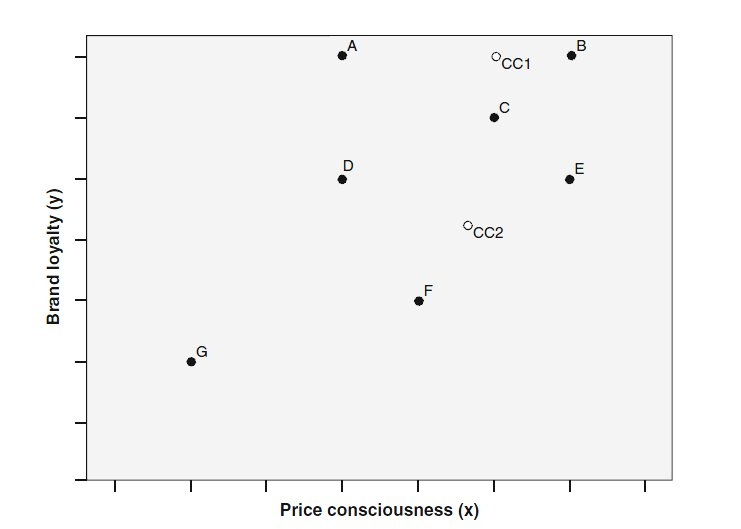
\includegraphics[scale=0.4]{images/kmeans1.jpg}\\
	\end{center}
\end{figure}
\begin{figure}[h!]
	\begin{center}
		% Requires \usepackage{graphicx}
		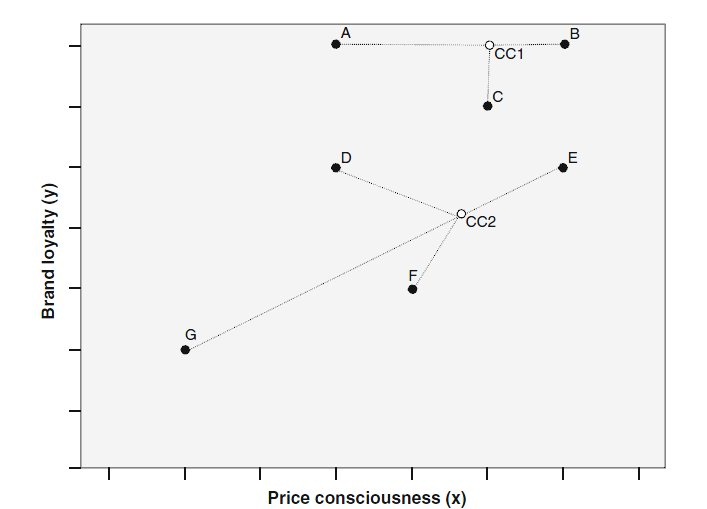
\includegraphics[scale=0.4]{images/kmeans2.jpg}\\
	\end{center}
\end{figure}
\begin{itemize}
\item Euclidean distances are computed from the cluster
centers to every single object. Each object is then assigned to the cluster center with
the shortest distance to it.

\item In this example, objects A, B, and C are
assigned to the first cluster, whereas objects D, E, F, and G are assigned to the
second. We now have our initial partitioning of the objects into two clusters.
\item Based on this initial partition, each cluster’s geometric center (i.e., its centroid)
is computed (third step). 
\item This is done by computing the mean values of the objects
contained in the cluster (e.g., A, B, C in the first cluster) regarding each of the variables
(in this example: price consciousness and brand loyalty).
\end{itemize}

\begin{figure}[h!]
	\begin{center}
		% Requires \usepackage{graphicx}
		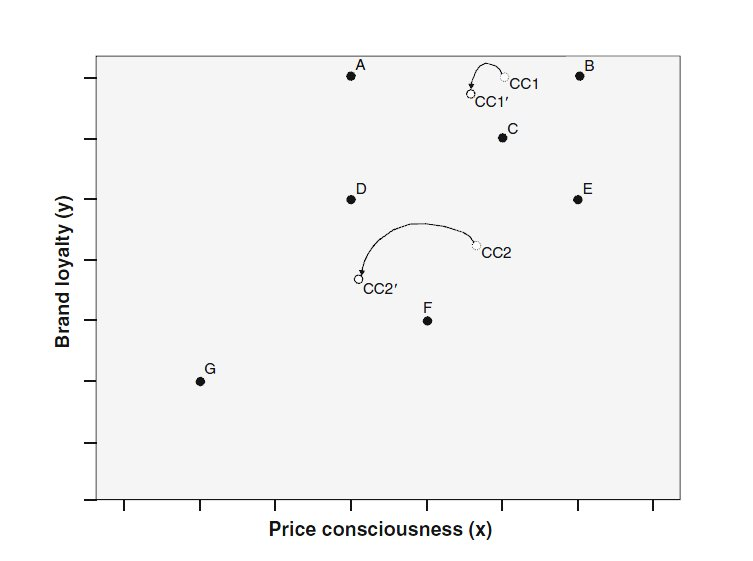
\includegraphics[scale=0.4]{images/kmeans3.jpg}\\
	\end{center}
\end{figure}
\begin{figure}[h!]
	\begin{center}
		% Requires \usepackage{graphicx}
		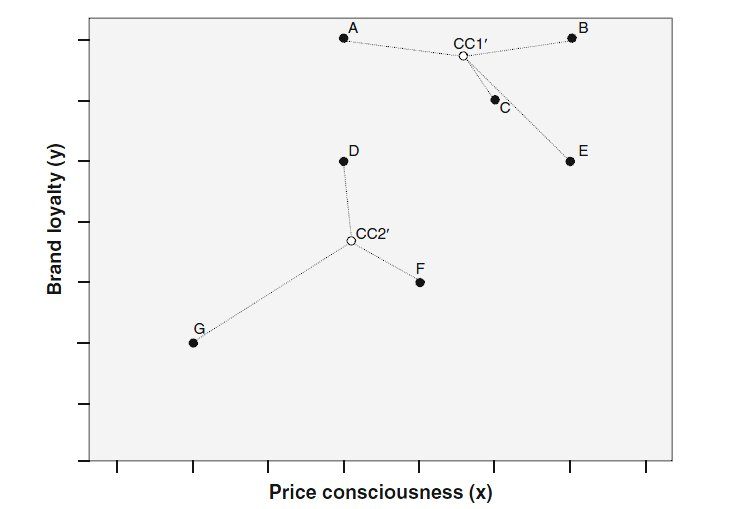
\includegraphics[scale=0.4]{images/kmeans4.jpg}\\
	\end{center}
\end{figure}
\begin{itemize}
\item Both clusters’centers now shift into new positions (CC1’ for the first and CC2’ for the second cluster).
\item In the fourth step, the distances from each object to the newly located cluster
centers are computed and objects are again assigned to a certain cluster on the basis
of their minimum distance to other cluster centers (CC1’ and CC2’).

\item Since the cluster centers’ position changed with respect to the initial situation in the first step,
this could lead to a different cluster solution. This is also true of our example, as
object E is now – unlike in the initial partition – closer to the first cluster center
(CC1’) than to the second (CC2’). Consequently, this object is now assigned to the
first cluster.
\item The k-means procedure now repeats the third step and
re-computes the cluster centers of the newly formed clusters, and so on.
In other words, steps 3 and 4 are repeated until a predetermined number of iterations are
reached, or convergence is achieved (i.e., there is no change in the cluster affiliations).
\end{itemize}

%============================================================================ %
\newpage
\subsection{Performance of k-means clustering}
Generally, k-means is superior to hierarchical methods as it is less affected by
outliers and the presence of irrelevant clustering variables. Furthermore, k-means
can be applied to very large data sets, as the procedure is less computationally
demanding than hierarchical methods. In fact, we suggest definitely using k-means
for sample sizes above 500, especially if many clustering variables are used. From
a strictly statistical viewpoint, k-means should only be used on interval or ratio-scaled
data as the procedure relies on Euclidean distances. However, the procedure is
routinely used on ordinal data as well, even though there might be some distortions.

One problem associated with the application of k-means relates to the fact that
the researcher has to pre-specify the number of clusters to retain from the data. This
makes k-means less attractive to some and still hinders its routine application in
practice.
\end{document}

%------------------------------------------------------------------%
\newpage
\section{Two-Step Cluster}
When you have a really large data set or you need a clustering procedure that can rapidly form clusters on the basis of either categorical or continuous data, neither of the previous two procedures are entirely appropriate. Hierarchical clustering requires a matrix of distances between all pairs of cases, and k-means requires shuffling cases in and out of clusters and knowing the number of clusters in advance.

The Two-Step Cluster Analysis procedure was designed for such applications. The name two-step clustering is already an indication that the algorithm is based on a two-stage approach: In the first stage, the algorithm undertakes a procedure that is very similar to the k-means algorithm. Based on these results, the two-step
procedure conducts a modified hierarchical agglomerative clustering procedure that
combines the objects sequentially to form homogenous clusters. This is done by
building a so-called \textbf{\textit{cluster feature tree}} whose \textbf{\textit{leaves}} represent distinct objects in the dataset. The procedure can handle categorical and continuous variables simultaneously
and offers the user the flexibility to specify the cluster numbers as well as
the maximum number of clusters, or to allow the technique to automatically choose
the number of clusters on the basis of statistical evaluation criteria.

The Two-Step Cluster Analysis requires only one pass of data
(which is important for very large data files).

Additionally, the procedure indicates each variable’s
importance for the construction of a specific cluster. These desirable features make
the somewhat less popular two-step clustering a viable alternative to the traditional
methods.
\subsection{Measures of Fit}
Two-Step Cluster Analysis guides the decision of how many clusters to retain from the data by
calculating measures-of-fit such as \textbf{\textit{Akaike’s Information Criterion (AIC)}} or \textbf{\textit{Bayes Information Criterion (BIC)}}.

These are relative measures of goodness-of-fit and are used to compare different
solutions with different numbers of segments.(``Relative" means that these criteria
are not scaled on a range of, for example, 0 to 1 but can generally take any value.)
Compared to an alternative solution with a different number of segments, smaller
values in AIC or BIC indicate an increased fit.

SPSS computes solutions for different
segment numbers (up to the maximum number of segments specified before) and
chooses the appropriate solution by looking for the smallest value in the chosen
criterion. However, which criterion should we choose? AIC is well-known for
overestimating the correct number of segments, while BIC has a slight tendency
to underestimate this number.

Thus, it is worthwhile comparing the clustering
outcomes of both criteria and selecting a smaller number of segments than
actually indicated by AIC. Nevertheless, when running two separate analyses,
one based on AIC and the other based on BIC, SPSS usually renders the same
results.
\end{document}

The clustering algorithm is based on a distance measure that gives the best results if all variables are independent, continuous variables have a normal distribution (or categorical variables have a multinomial distribution). This is seldom the case in practice, but the algorithm is thought to behave reasonably well when the assumptions are not met.

Because cluster analysis does not involve hypothesis testing and calculation of observed significance levels, other than for descriptive follow-up, it's perfectly acceptable to cluster data that may not meet the assumptions for best performance.

The final outcome may depend on the order of the cases in the file. To minimize the effect, arrange the cases in random order. Sort them by the last digit of their ID numbers or something similar.

\subsection{Step 1: Pre-clustering: Making Little Clusters}
The first step of the two-step procedure is formation of pre-clusters. The goal of pre-clustering is to reduce the size of the Distance matrix (the matrix that contains distances between all
possible pairs of cases). Pre-clusters are just clusters of the original cases that are used in place of the raw data in the hierarchical clustering. As a case is read, the algorithm
decides, based on a distance measure, if the current case should be merged with a previously formed pre-cluster or start a new precluster.

When preclustering is complete, all cases in the same precluster are treated as a single entity. The size of the distance matrix is no longer dependent on the number of cases but on the number of preclusters.

\subsection{Step 2: Hierarchical Clustering of Preclusters}
In the second step, SPSS uses the standard hierarchical clustering algorithm on the
preclusters. Forming clusters hierarchically lets you explore a range of solutions with
different numbers of clusters.
Tip: The Options dialog box lets you control the number of preclusters. Large numbers
of preclusters give better results because the cases are more similar in a precluster;
however, forming many preclusters slows the algorithm.

Some of the options you can specify when using two-step clustering are:
\textbf{Standardization:} The algorithm will automatically standardize all of the variables
unless you override this option.

\textbf{Distance measures:} If your data are a mixture of continuous and categorical variables,
you can use only the log-likelihood criterion. The distance between two clusters
depends on the decrease in the log-likelihood when they are combined into a single
cluster. If the data are only continuous variables, you can use the Euclidean
distance between two cluster centers. Depending on the distance measure selected,
cases are assigned to the cluster that leads to the largest log-likelihood or to the cluster
that has the smallest Euclidean distance.


\textbf{Number of clusters:} You can specify the number of clusters to be formed, or you can let
the algorithm select the optimal number based on either the Schwarz Bayesian
Criterion or the Akaike information criterion.


\textbf{Outlier handling:} You have the option to create a separate cluster for cases that don't fit
well into any other cluster.


\textbf{Range of solutions:} You can specify the range of cluster solutions that you want to see.

\end{document} 
